\documentclass[../main.tex]{subfiles}

\begin{document}

\section{排中律と否定}

前章では，命題 \(A\) とその否定 \(\sim A\) について，矛盾律と排中律を確認した。本章では，集合の図を用いて排中律をもう少し詳しく考える。古典論理では，ある命題 \(A\) について，\(A\) であるか，または \(A\) でないかのどちらかが必ず成り立つと考える。これが排中律である。

\begin{center}
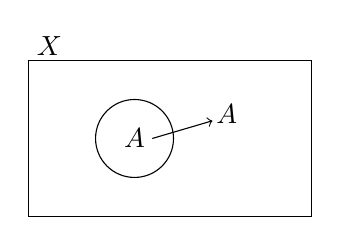
\begin{tikzpicture}[scale=0.9]
  \draw (0,0) rectangle (4,2.2);
  \node at (0.3,2.4) {\(X\)};
  \draw (1.5,1.1) circle (0.55);
  \node at (1.5,1.1) {\(A\)};
  \draw[->] (1.75,1.1) -- (2.6,1.35);
  \node at (2.8,1.45) {\(A\)};
\end{tikzpicture}
\end{center}

全体集合を \(X\)，その部分集合を \(A\) とすると，古典的な集合論では
\[
  A \cup \overline{A} = X
\]
が成り立つ。これは，任意の対象が \(A\) に属するか，または \(A\) に属しないかのどちらかである，という排中律に対応する。

しかし，\(A\) の境界があいまいである場合，排中律がそのまま成立すると言えるかは問題になる。たとえば，「背が高い」「若い」のような述語では，どこまでを \(A\) とし，どこからを \(\overline{A}\) とするかが明確でない。このような場合，古典論理の排中律を適用するには，あらかじめ境界を明確に定める必要がある。

\begin{sidebox}[TBred]{注意}
  \(A\) の境界があいまいな場合，\(A \cup \overline{A}=X\) と言えるかどうかは自明でない。これは排中律の適用範囲に関わる問題である。
\end{sidebox}

否定に関するもう1つの重要な法則は，二重否定律である。
\[
  \sim\sim A = A
\]
これは，\(A\) でないことはない，ということから \(A\) を導く規則である。古典論理では二重否定律が認められるが，直観主義論理のようにこれを一般には認めない体系もある。

\subsection{背理法}

背理法は，ある命題 \(A\) を証明するために，いったん \(\sim A\) を仮定し，そこから矛盾を導く方法である。矛盾が導かれれば，\(\sim A\) は成り立たない。古典論理では，そこから二重否定律を用いて \(A\) を結論する。

たとえば，\(\sqrt{2}\) が有理数でないことは
\[
  \sqrt{2} \neq \frac{a}{b}
  \qquad
  (a,b \in \mathbb{N})
\]
を示す問題として表される。背理法では，まず反対に
\[
  \sqrt{2} = \frac{a}{b}
\]
であると仮定する。そこから整数 \(a,b\) の偶奇に関する矛盾を導くことで，仮定が誤りであることを示す。

背理法の構造は次のように整理できる。
\[
  \begin{array}{c}
    \text{仮定} \\
    \dfrac{a}{b} \\
    \downarrow \\
    \text{矛盾}
  \end{array}
\]
より一般には，
\[
  \begin{array}{c}
    A \\
    \sim A \\
    \downarrow \\
    \text{矛盾}
  \end{array}
\]
という形で表される。ここで \(\sim A\) から矛盾が出るなら，\(\sim\sim A\) が得られる。古典論理では
\[
  \frac{\sim\sim A}{A}
\]
という推論が許されるため，最終的に \(A\) を結論できる。

\begin{sidebox}[TBred]{注意}
  背理法で \(\sim\sim A\) から \(A\) を導く段階では，排中律または二重否定律が必要になる。この点が，古典論理と直観主義論理を分ける重要な箇所である。
\end{sidebox}

\section{完備ブール代数の演算規則}

完備ブール代数では，和 \(+\)，積 \(\times\)，補元 \(-x\)，最小元 \(0\)，最大元 \(1\) が互いに整合するように定義される。ここでは，これまでに出てきた演算規則をまとめる。

\subsection{モジュラ律}

順序関係 \(x \leq y\) が成り立つとき，\(x\) は \(y\) に含まれているものとして考えられる。このとき，和と積は次のように簡約される。
\[
  x \leq y
  \quad \Rightarrow \quad
  x + y = y
  \quad \text{かつ} \quad
  x \times y = x
\]
和では大きい方の \(y\) が残り，積では小さい方の \(x\) が残る。

\begin{sidebox}[TBred]{講義メモ}
  元資料には「かぶりならば」と読めるメモがある。ここでは，\(x\) が \(y\) に含まれている場合，重なりを取ると \(x\)，合わせると \(y\) になる，という意味として整理する。
\end{sidebox}

\subsection{交換律}

任意の \(x,y\) について，
\[
  x + y = y + x
\]
\[
  x \times y = y \times x
\]
が成り立つ。和と積はいずれも，左右の順序を入れ替えても結果が変わらない。

\subsection{結合律}

任意の \(x,y,z\) について，
\[
  (x+y)+z = x+(y+z)
\]
\[
  (x \times y) \times z = x \times (y \times z)
\]
が成り立つ。したがって，3つ以上の元の和や積を取るとき，括弧の付け方を変えても結果は変わらない。

\subsection{分配律}

和と積のあいだには，次の2つの分配律が成り立つ。
\[
  x \times (y+z)
  =
  (x \times y) + (x \times z)
\]
\[
  x + (y \times z)
  =
  (x+y) \times (x+z)
\]
これは，集合でいえば共通部分と和集合の分配法則に対応する。

\subsection{補元律}

補元 \(-x\) は，\(x\) と重ならず，かつ \(x\) と合わせると全体になる元である。そのため，
\[
  x \times -x = 0
\]
\[
  x + -x = 1
\]
が成り立つ。

\begin{sidebox}[TBred]{講義メモ}
  「極限に一番近い前提，etc はつけない」と読めるメモがある。補元を定義するときは，単に \(x\) と交わらない任意の元ではなく，条件を満たす最大の元を取る点が重要である。
\end{sidebox}

\subsection{ド・モルガン律}

ド・モルガン律は，和と積に対する否定の分配を表す。
\[
  -(x+y) = -x \times -y
\]
\[
  -(x \times y) = -x + -y
\]
和の否定は否定どうしの積になり，積の否定は否定どうしの和になる。

\subsection{二重否定律}

任意の \(x\) について，
\[
  --x = x
\]
が成り立つ。これは，命題論理における \(\sim\sim A=A\) に対応する。

\subsection{単位元・零元}

和と積において，\(0\) と \(1\) は次のように振る舞う。
\[
  x+0=x,
  \qquad
  x+1=1,
  \qquad
  x \times 0=0,
  \qquad
  x \times 1=x
\]
和において \(0\) は単位元，\(1\) は吸収元である。積において \(1\) は単位元，\(0\) は吸収元である。

\section{\texorpdfstring{\(0\)}{0} と \texorpdfstring{\(1\)}{1} に関する計算}

\subsection{\texorpdfstring{\(0\)}{0} と \texorpdfstring{\(1\)}{1} の否定}

補元の定義より，最小元 \(0\) と最大元 \(1\) は互いに否定の関係にある。
\[
  -0 = 1,
  \qquad
  -1 = 0
\]

\subsection{\texorpdfstring{\(0\)}{0} と \texorpdfstring{\(1\)}{1} の演算}

和については，次が成り立つ。
\[
  0+0=0,
  \qquad
  0+1=1,
  \qquad
  1+1=1,
  \qquad
  1+0=1
\]
積については，次が成り立つ。
\[
  0 \times 0 = 0,
  \qquad
  0 \times 1 = 0,
  \qquad
  1 \times 1 = 1,
  \qquad
  1 \times 0 = 0
\]
これらは，命題論理の真理値計算において，\(0\) を偽，\(1\) を真と見なすときの基本規則になる。

\end{document}
